\documentclass[a4paper]{article}
\usepackage{geometry}
\usepackage{graphicx}
\usepackage{natbib}
\usepackage{amsmath}
\usepackage{amssymb}
\usepackage{amsthm}
\usepackage{paralist}
\usepackage{epstopdf}
\usepackage{tabularx}
\usepackage{longtable}
\usepackage{multirow}
\usepackage{multicol}
\usepackage[hidelinks]{hyperref}
\usepackage{fancyvrb}
\usepackage{algorithm}
\usepackage{algorithmic}
\usepackage{float}
\usepackage{paralist}
\usepackage[svgname]{xcolor}
\usepackage{enumerate}
\usepackage{array}
\usepackage{times}
\usepackage{url}
\usepackage{fancyhdr}
\usepackage{comment}
\usepackage{environ}
\usepackage{times}
\usepackage{textcomp}
\usepackage{caption}


\urlstyle{rm}

\setlength\parindent{0pt} % Removes all indentation from paragraphs
\theoremstyle{definition}
\newtheorem{definition}{Definition}[]
\newtheorem{conjecture}{Conjecture}[]
\newtheorem{example}{Example}[]
\newtheorem{theorem}{Theorem}[]
\newtheorem{lemma}{Lemma}
\newtheorem{proposition}{Proposition}
\newtheorem{corollary}{Corollary}

\floatname{algorithm}{Procedure}
\renewcommand{\algorithmicrequire}{\textbf{Input:}}
\renewcommand{\algorithmicensure}{\textbf{Output:}}
\newcommand{\abs}[1]{\lvert#1\rvert}
\newcommand{\norm}[1]{\lVert#1\rVert}
\newcommand{\RR}{\mathbb{R}}
\newcommand{\CC}{\mathbb{C}}
\newcommand{\Nat}{\mathbb{N}}
\newcommand{\br}[1]{\{#1\}}
\DeclareMathOperator*{\argmin}{arg\,min}
\DeclareMathOperator*{\argmax}{arg\,max}
\renewcommand{\qedsymbol}{$\blacksquare$}

\definecolor{dkgreen}{rgb}{0,0.6,0}
\definecolor{gray}{rgb}{0.5,0.5,0.5}
\definecolor{mauve}{rgb}{0.58,0,0.82}

\newcommand{\Var}{\mathrm{Var}}
\newcommand{\Cov}{\mathrm{Cov}}

\newcommand{\vc}[1]{\boldsymbol{#1}}
\newcommand{\xv}{\vc{x}}
\newcommand{\Sigmav}{\vc{\Sigma}}
\newcommand{\alphav}{\vc{\alpha}}
\newcommand{\muv}{\vc{\mu}}

\newcommand{\red}[1]{\textcolor{red}{#1}}

\def\x{\mathbf x}
\def\y{\mathbf y}
\def\w{\mathbf w}
\def\v{\mathbf v}
\def\E{\mathbb E}
\def\V{\mathbb V}

% TO SHOW SOLUTIONS, include following (else comment out):
\newenvironment{soln}{
    \leavevmode\color{blue}\ignorespaces
}{}


\hypersetup{
%    colorlinks,
    linkcolor={red!50!black},
    citecolor={blue!50!black},
    urlcolor={blue!80!black}
}

\geometry{
  top=1in,            % <-- you want to adjust this
  inner=1in,
  outer=1in,
  bottom=1in,
  headheight=3em,       % <-- and this
  headsep=2em,          % <-- and this
  footskip=3em,
}


\pagestyle{fancyplain}
\lhead{\fancyplain{}{Homework 3}}
\rhead{\fancyplain{}{CS 760 Machine Learning}}
\cfoot{\thepage}

\title{\textsc{Homework 3}} % Title

%%% NOTE:  Replace 'NAME HERE' etc., and delete any "\red{}" wrappers (so it won't show up as red)

\author{
$>>$Sean(Xiaoyu) Sun$<<$ \\
$>>$9078202463$<<$\\
} 

\date{}

\begin{document}

\maketitle 


\textbf{Instructions:} 
Although this is a programming homework, you only need to hand in a pdf answer file.
There is no need to submit the latex source or any code.
You can choose any programming language, as long as you implement the algorithm from scratch. 

Use this latex file as a template to develop your homework.
Submit your homework on time as a single pdf file to Canvas.
Please check Piazza for updates about the homework.

\section{A Simplified 1NN Classifier}
You are to implement a 1-nearest-neighbor learner for classification.
To simplify your work, your program can assume that
\begin{itemize}
\item each item has $d$ continuous features $\x \in \RR^d$
\item binary classification and the class label is encoded as $y \in \{0,1\}$
\item data files are in plaintext with one labeled item per line, separated by whitespace:
$$x_{11} \quad \ldots \quad x_{1d} \quad y_1$$
$$...$$
$$x_{n1} \quad \ldots \quad x_{nd} \quad y_n$$
\end{itemize}

Your program should implement a 1NN classifier: 
\begin{itemize}
\item Use Mahalanobis distance $d_A$ parametrized by a positive semidefinite (PSD) diagonal matrix $A$.  For $\x, \x' \in \RR^d$,
$$d_A(\x,\x') = \|\x-\x'\|_A = \sqrt{(\x-x')^\top A (\x-x')}.$$
We will specify $A$ in the questions below. (Hint: $d$ is dimension while $d_A$ with a subscript is distance)
\item If multiple training points are the equidistant nearest neighbors of a test point, you may use any one of those training points to predict the label.
\item You do not have to implement kd-tree.
\end{itemize}

\section{Questions}
\begin{enumerate}

\item (5 pts) What is the mathematical condition on the diagonal elements for a diagonal matrix $A$ to be PSD?
\begin{soln}  
For every real vector $x$, when ${x^{T}}Ax =  \sum_{i=1}^n {{x_{i}^{2}}A_{i} } >= 0$, A is PSD. So every element $a_{ii}$ in A need to be non-negative to make A a PSD matrix. 
\end{soln}

\item (5 pts) Given a training data set $D$, how do we preprocess it to make each feature dimension mean 0 and variance 1? (Hint: give the formula for $\hat \mu_j, \hat \sigma_j$ for each dimension $j$, and explain how to use them to normalize the data.  You may use either the $1 \over n$ or $1 \over n-1$ version of sample variance.  You may assume the sample variances are non-zero.) 

\begin{soln}  
To make each feature dimension mean 0 and variance 1, we need to use $x_{di}' = \frac{x_{di}-\hat \mu_d}{\hat \sigma_d}$ for every feature dimension d.
\end{soln}


\item (5 pts) Let $\tilde \x$ be the preprocessed data. Give the formula for the Euclidean distance between $\tilde \x, \tilde \x'$.

\begin{soln}  
$D_{Euclidean}(\tilde \x, \tilde \x') = \sqrt{\sum_{i=1}^n (\tilde \x_{i} - \tilde \x_{i}')^{2}} $ where i is the $i^{th}$ dimension of x
\end{soln}


\item (5 pts) Give the equivalent Mahalanobis distance on the original data $\x, \x'$ by specifying $A$. (Hint: you may need $\hat \mu_j, \hat \sigma_j$)

\begin{soln}  
 $D_{Mahalanobis}(\x, \x') = \sqrt{(\x -  \x')^{T}A(\x -  \x')} = \sqrt{\sum_{i=1}^n (\x_{i} -  \x_{i}')^{2}a_{ii}} $\\
$D_{Euclidean}(\tilde \x, \tilde \x') = \sqrt{\sum_{i=1}^n (\tilde \x_{i} - \tilde \x_{i}')^{2}} = \sqrt{\sum_{i=1}^n (\frac{\x_{i}-\hat\mu_i}{\hat \sigma_i} - \frac{\x_{i}'-\hat\mu_i}{\hat \sigma_i})^{2}} = \sqrt{\sum_{i=1}^n (\frac{\x_{i}-\x'_{i}}{\hat \sigma_i} )^{2}}$\\

To make $D_{Euclidean}(\tilde \x, \tilde \x') = D_{Mahalanobis}(\x, \x') $, every $a_{ii}$ in A need to be equal to $\frac{1}{\hat \sigma_i}^{2}$
\end{soln}


\item (5 pts) Let the diagonal elements of $A$ be $a_{11}, \ldots, a_{dd}$.
Define a diagonal matrix $L$ with diagonal $\sqrt{a_{11}}, \ldots, \sqrt{a_{dd}}$.
Define $\tilde \x = L\x$.
Prove that $d_I(\tilde \x, \tilde \x') = d_A(\x, \x')$ where $I$ is the identity matrix.

\begin{soln}  
$D_{I}(\tilde \x, \tilde \x') = \sqrt{\sum_{i=1}^n (\tilde \x_{i} - \tilde \x_{i}')^{2}} = \sqrt{\sum_{i=1}^n (\sqrt{a_{ii}}\x_{i} - \sqrt{a_{ii}}\x_{i}')^{2}}  = \sqrt{\sum_{i=1}^n {a_{ii}}(\x_{i} - \x_{i}')^{2}} $\\
$D_{A}(\x, \x') = \sqrt{(\x -  \x')^{T}A(\x -  \x')} = \sqrt{\sum_{i=1}^n (\x_{i} -  \x_{i}')^{2}a_{ii}}$\\

So, $D_{I}(\tilde \x, \tilde \x') = D_{A}(\x, \x')$
\end{soln}


\item (5 pts) Geometrically, what does $L\x$ do to the point $\x$?  Explain in simple English.

\begin{soln}  
$L\x $ changes every feature dimension's magnitude. In other words, by applying $L\x$, we can enlarge or condense the value space for every feature by using different $a_{ii}$. To my uderstanding, $L\x$ can be considered as weight vector.
\end{soln}


\item (10 pts) Let $U$ be any orthogonal matrix.
Define $\tilde \x = UL\x$.
(i) Prove that $d_I(\tilde \x, \tilde \x') = d_A(\x, \x')$ again. 
(ii) Geometrically, what does $UL\x$ do to the point $\x$?  Explain in simple English.

\begin{soln}  
(i).\\
$D_{I}(\tilde \x, \tilde \x') = \sqrt{(\tilde \x - \tilde \x')^{T}I(\tilde \x - \tilde \x')} =   \sqrt{(\x -\x')^{T}L^{T}U^{T}UT(\x - \x')} $\\
Since $U$ is orthognal matrix, $U^{T}U = I$ and $L^{T}IL = A$.\\ So $D_{I}(\tilde \x, \tilde \x') =  \sqrt{(\x -  \x')^{T}A(\x -  \x')} = D_{A}(\x, \x') $

(ii).\\
Still,$ L\x$  changes feature's magnitude. By applying orthognal matrix on the left side, we can rotate feature values to a new coordinates without changing the relative Euclidean distance between every corrdinates.
\end{soln}



\item (20 pts) Use the whole D2z.txt as training set.  Use Euclidean distance (i.e. $A=I$).
Visualize the predictions of 1NN on a 2D grid $[-2:0.1:2]^2$.
That is, you should produce test points whose first feature goes over $-2, -1.9, -1.8, \ldots, 1.9, 2$, so does the second feature independent of the first feature.
You should overlay the training set in the plot, just make sure we can tell which points are training, which are grid.

\begin{soln}  
	   \begin{figure}[H]
	        \centering
	        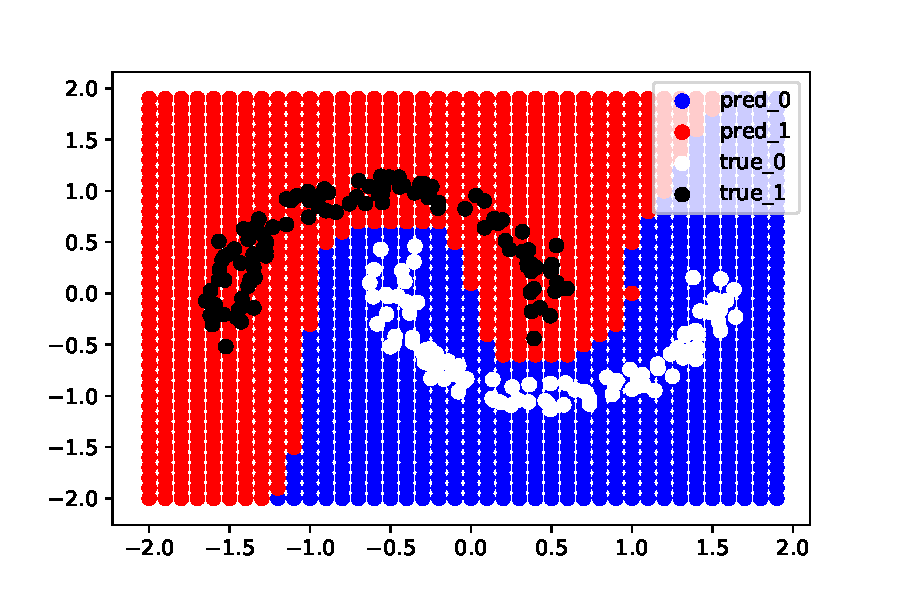
\includegraphics[width=0.6\textwidth]{question8.pdf}
	        \captionsetup{labelformat=empty}
	        \caption{}
	        \label{fig:my_label}
	   \end{figure}
\end{soln}

\item (To normalize, or not to normalize?)
Start from D2a.txt.  Perform 5-fold cross validation.
  \begin{enumerate}
  \item (5 pts) Do not normalize the data.  Report 1NN cross validation error rate for each fold, then the average (that's 6 numbers). 

\begin{soln}  
validaiton errors are all zero. The average error is also zero.
\end{soln}

  \item (5 pts) Normalize the data.  Report 1NN cross validation error rate (again 6 numbers).  (Hints: Do not normalize the labels!  The relevant quantities should be estimated from the training portion, but applied to both training and validation portions.  This should happen 5 times.  Also, you would either change $\x$ into $\tilde \x = L\x$ but then use Euclidean distance on $\tilde \x$, or do not change $\x$ but use an appropriate $A$; don't mix the two.)

\begin{soln}  
validaiton errors are [0.075, 0.075, 0.1, 0.05, 0.05]. The average error is 0.07.
\end{soln}

  \item (5 pts) Look at D2a.txt, explain the effect of normalization on CV error.  Hint: the first 4 features are different than the next 2 features.

\begin{soln}  
Values for the first 4 features are much smaller than values of the last two features. And the last two features are more important than the first 4 features for making prediction. So without normalization, my 1NN model gives perfect predictions. But after applying normalization, the weights of every features are balaned, which means the model focuses less on the last two important features and focuses more on the first 4 trivial features. That could be the reason why applying normalization leads to worse result.
\end{soln}

  \end{enumerate}

\item (Again.  10 pts)
Repeat the above question, starting from D2b.txt.

\begin{soln} 
For original dataset: validation errors are [0.275, 0.175, 0.15, 0.175, 0.2], the average error is 0.195.\\
For normalized dataset: validaiton errors are all zero. The average error is also zero.

Similar to D2a, D2b also has unbalanced feature values. The second feature has much larger value than the first one. However, normalization gives better result this time. My hypohthesis here is that, though having different magnitudes, this two features are equally important for making prediction. So normalization balances the weights of these two features and thus leads to a better result.
\end{soln}

\item (5 pts) What do you learn from Q9 and Q10?


\begin{soln}  
We should be careful about normalization. Some datasets should be normalized to get better result but some should not be normalized to keep the natural feature weights. In other words, we should be careful about features' weights (or importance) when doing pre-processing. 
\end{soln}

\item (Weka, 10 pts)
Repeat Q9 and Q10 with Weka.
Convert appropriate data files into ARFF format.
Choose classifiers / lazy / IBk.
Set $K=1$.
Choose 5-fold cross validation.
Let us know what else you needed to set.  Compare Weka's results to your Q9 and Q10.

\begin{soln}
D2a: 0.085\\
D2a\_norm(Weka normalized version): 0.055\\
D2a\_norm(my own normalized version): 0.055 \\
D2b: 0.05\\
D2b\_norm(Weka normalized version): 0.00\\
D2b\_norm(My own normalized version): 0.00

"Weka normalized version"  means applying the "Normalize" fliter in preprcoessing module inside Weka on the orginal D2a and D2b datasets.
I notice that passing normalized version and unnormalized dataset give same resutls for both datasets D2a and D2b.\\
Weka's D2a results are different from what I got by using my 1NN model on unnormalizaed data but it's close to my normalized D2a result,  and its D2b results is same as my normalized D2b result.
So based on this, my guess about this result is that Weka applies auto-normalization to datasets.
\end{soln}

\end{enumerate}

\bibliographystyle{apalike}
\end{document}
